\documentclass[../main]{subfiles}
\begin{document}

\chapter{时分复用与解复用}%
\label{cha:tdfm}

% \section{实验目的}%
% \label{sec:\arabic{chapter}aim}
%
% \begin{itemize}
%   \item 掌握时分复用的概念及工作原理。
%   \item 了解时分复用在整个通信系统中的作用。
% \end{itemize}
%
% \section{实验器材}%
% \label{sec:\arabic{chapter}equipment}
%
% \begin{table}[htbp]
%   \centering
%   \caption{实验器材}%
%   \label{tab:\arabic{chapter}equipment}
%   \csvautobooktabular[respect percent]{tab/\arabic{chapter}equipment.csv}
% \end{table}
%
\section{实验原理}%
\label{sec:\arabic{chapter}principle}

\begin{figure}[htbp]
  \centering
  \begin{subfigure}[htbp]{\linewidth}
    \centering
    \includegraphics[
      width = \linewidth,
    ]{\arabic{chapter}dia/tdfm}
    \caption{256K 时分复用}%
    \label{fig:\arabic{chapter}diatdfm}
  \end{subfigure}

  \begin{subfigure}[htbp]{\linewidth}
    \centering
    \includegraphics[
      width = \linewidth,
    ]{\arabic{chapter}dia/itdfm}
    \caption{256K 解时分复用}%
    \label{fig:\arabic{chapter}diaitdfm}
  \end{subfigure}
  \caption{实验原理框图}%
  \label{fig:\arabic{chapter}dia}
\end{figure}

对于 2048K 时分复用和解复用实验,其实验框
图~\ref{fig:\arabic{chapter}diatdfm}和 256K 时分复用和解复用实验框
图~\ref{fig:\arabic{chapter}diaitdfm}基本一致。

21 号模块的 PCM 数据和 2 号模块的数字终端数据,经过 7 号模块进行 256K 时分复
用和解复用后,再送入到相应的 PCM 译码单元和 2 号终端模块。时分复用是将各路输
入变为并行数据。然后,按给端口数据所在的时隙进行帧的拼接,变成一个完整的数据
帧。最后,并串变换将数据输出。解复用的过程是先提取帧同步,然后将一帧数据缓存
下来。接着按时隙将帧数据解开,最后,每个端口获取自己时隙的数据进行并串变换输
出。

此时 256K 时分复用与解复用模式下,复用帧结构为:第 0 时隙是巴克码帧头、第1--3
时隙是数据时隙,其中第 1 时隙输入的数字信号源,第 2 时隙输入的 PCM 数据,第 3
时隙由 7 号模块自带的拨码开关 S1 的码值作为数据。

\section{实验步骤}%
\label{sec:\arabic{chapter}procedure}

\subsection{256K 时分复用帧信号观测}%
\label{sub:tdfm}

% 该项目是通过观测 256K 帧同步信号及复用输出波形,了解复用的基本原理。

% \begin{table}[htbp]
%   \centering
%   \caption{连线}%
%   \label{tab:\arabic{chapter}\arabic{subsection}}
%   \csvautobooktabular[respect percent]{tab/\arabic{chapter}\arabic{subsection}.csv}
% \end{table}

% \begin{enumerate}
%   \item 关电,按表~\ref{tab:\arabic{chapter}\arabic{subsection}}所示进行连线
%     。
%   \item 开电,设置主控菜单,选择【主菜单】→【通信原理】→【时分复用】→【复用速率 256KHz】。
%   \item 此时系统初始状态为:在复用时隙的速率 256K 模式,7 号模块的复用信号只
%     有四个时隙,其中第 0、1、2、3 输出数据分别为巴克码、DIN1、DIN2、开关 S1
%     拨码信号。
%   \item 实验操作及波形观测。
\begin{enumerate}
  \item 帧同步码观测:用示波器探头接 7 号模块的 TH10 复用输出,观测帧头的
    巴克码图~\ref{fig:tdfm/barkker}和图~\ref{fig:tdfm/barkker0}。

    % 注:为方便记录巴克码波形,可先将 7 号模块上的拨码开关 S1 全置为 0,使
    % 整个复用中只有帧同步信号。

  \item 帧内 PN 序列信号观测

    关电继续连线,将信号源的 PN 连接到 7 号模块的 DIN1,即将 PN15 送至第
    1 时隙。通电,用示波器探头接 7 号模块的 TH10 复用输出,需要用数字示波
    器的存储功能观测 3 个周期中的第 1 时隙的信号如图~\ref{fig:pn}。
\end{enumerate}
% \end{enumerate}

\begin{figure}[htbp]
  \centering
  \begin{subfigure}[htbp]{0.45\linewidth}
    \centering
    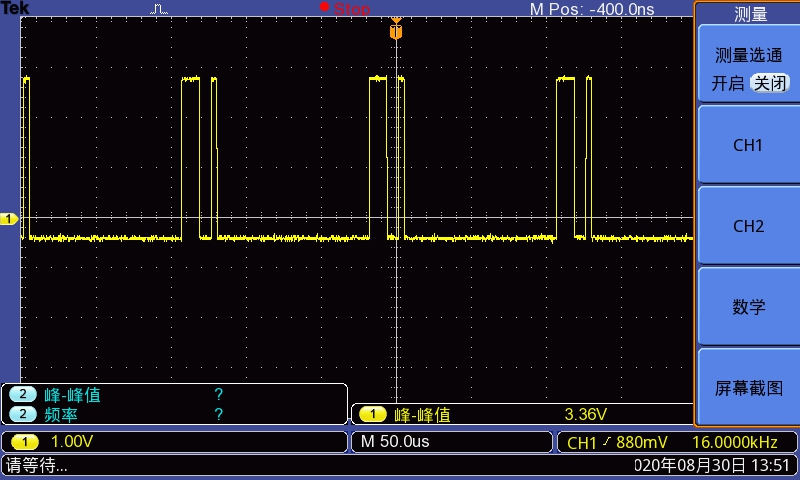
\includegraphics[
      width = \linewidth,
    ]{tdfm/barkker0}
    \caption{拨码开关 S1 全置为 0时的巴克码}%
    \label{fig:tdfm/barkker0}
  \end{subfigure}
  \quad
  \begin{subfigure}[htbp]{0.45\linewidth}
    \centering
    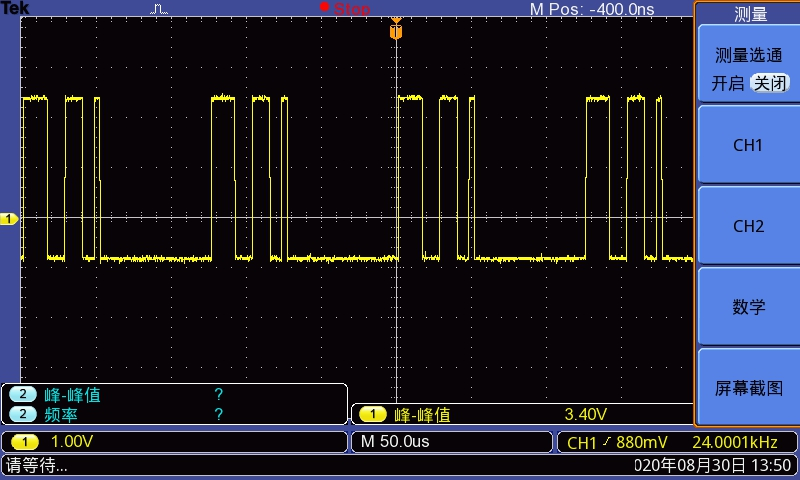
\includegraphics[
      width = \linewidth,
    ]{tdfm/barkker}
    \caption{巴克码}%
    \label{fig:tdfm/barkker}
  \end{subfigure}

  \begin{subfigure}[htbp]{0.45\linewidth}
    \centering
    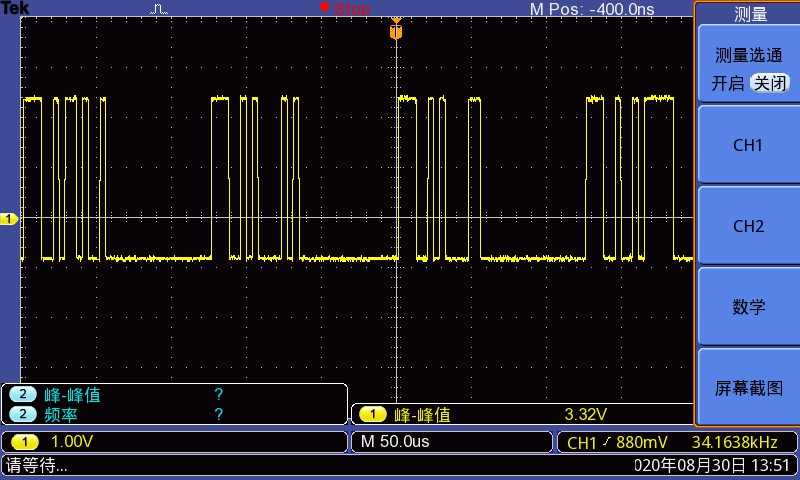
\includegraphics[
      width = \linewidth,
    ]{pn}
    \caption{PN}%
    \label{fig:pn}
  \end{subfigure}
  \caption{时分复用}%
  \label{fig:tdfm}
\end{figure}

\begin{Exercise}[title = 思考]
  PN15 序列的数据是如何分配到复用信号中的?
\end{Exercise}

\begin{Answer}
  PN15 序列 00010011010111 分成了长度为8的子序列插入到了复用信号中。不足8的子
  序列由下一个 PN15 序列补齐。
\end{Answer}

\subsection{256K 时分复用及解复用}%
\label{sub:256k}

% 该项目是将模拟信号通过 PCM 编码后,送到复用单元,再经过解复用输出,最后译码输
% 出。

% \begin{table}[htbp]
%   \centering
%   \caption{连线}%
%   \label{tab:\arabic{chapter}\arabic{subsection}}
%   \csvautobooktabular[respect percent]{tab/\arabic{chapter}\arabic{subsection}.csv}
% \end{table}

% \begin{enumerate}
%   \item 关电,按表~\ref{tab:\arabic{chapter}\arabic{subsection}}所示进行连线。
%   \item 开电,设置主控菜单,选择【主菜单】→【通信原理】→【时分复用】→【复用速
%     率 256KHz】。将模块 13 的 S3 拨位“0100”。将 21 号模块的开关 S1 拨至 A-LAW
%     (或 U-LAW)。
%   \item 此时系统初始状态为:在复用时隙的速率 256K 模式,7 号模块的复用信号只
%     有四个时隙,其中第 0、1、2、3 输出数据分别为巴克码、DIN1、DIN2、开关 S1
%     拨码信号。其中,信号源 A-OUT 输出设置为 1KHz 的正弦波,幅度由 W1 可调(频
%     率和幅度参数可根据主控模块操作说明进行调节);7 号模块的 DIN2 端口送入
%     PCM 数据。正常情况下,7 号模块的“同步”指示灯亮。
%
%     注:若发现“失步”或“捕获”指示灯亮,先检查连线或拨码是否正确,再逐级观测数
%     据或时钟是否正常。
%   \item 实验操作及波形观测。
\begin{enumerate}
  \item 帧内编码信号观测

    将 PCM 信号输入 DIN2,观测复用输出的数据。

    \begin{Exercise}[title = 思考]
      将连续三帧的各时隙的内容填入表~\ref{tab:itdfm}中,并进行简单的说明分析
      。
    \end{Exercise}

    \begin{Answer}
      TS0 是巴克码,TS1 是 PN15 码的一半,TS2 是 PCM 码,TS3 是拨码开关的输入
      。
    \end{Answer}

    \begin{table}[htbp]
      \centering
      \caption{帧内编码信号观测}%
      \label{tab:itdfm}
      \csvautobooktabular[respect percent]{tab/itdfm.csv}
    \end{table}

    % 注:PCM 复用后会有两帧的延时。

    \begin{Exercise}[title = 思考]
      PCM 数据是如何分配到复用信号中去的?
    \end{Exercise}

    \begin{Answer}
      PCM 序列直接插入到了复用信号的时隙 TS1 中。
    \end{Answer}

  \item 帧同步信号观测

    观测 TH11(FSIN)、TH7(FSOUT)的时序关系图~\ref{fig:fs}。

    \begin{Exercise}
      分析为何要使用 FSOUT 作为模块 21 的译码帧同步信号。
    \end{Exercise}

    \begin{Answer}
      FSOUT 为解复用模块提取帧同步,与解复用后的 PCM 信号在时间上对齐,可用于
      PCM 译码。
    \end{Answer}

  \item 解复用 PCM 信号观测

    对比观测复用前与解复用后的 PCM 序列图~\ref{fig:pcm/fm}。对比观测 PCM 编译
    码前后的正弦波信号图~\ref{fig:pcm/encode}。
\end{enumerate}
% \end{enumerate}

\begin{figure}[htbp]
  \centering
  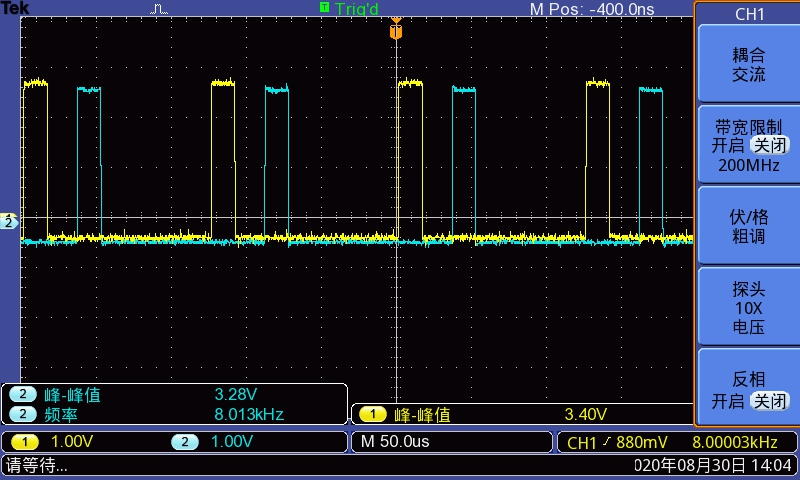
\includegraphics[
    width = 0.8\linewidth,
  ]{fs}
  \caption{FSOUT 对比 FSIN}%
  \label{fig:fs}
\end{figure}

\begin{figure}[htbp]
  \centering
  \begin{subfigure}[htbp]{0.45\linewidth}
    \centering
    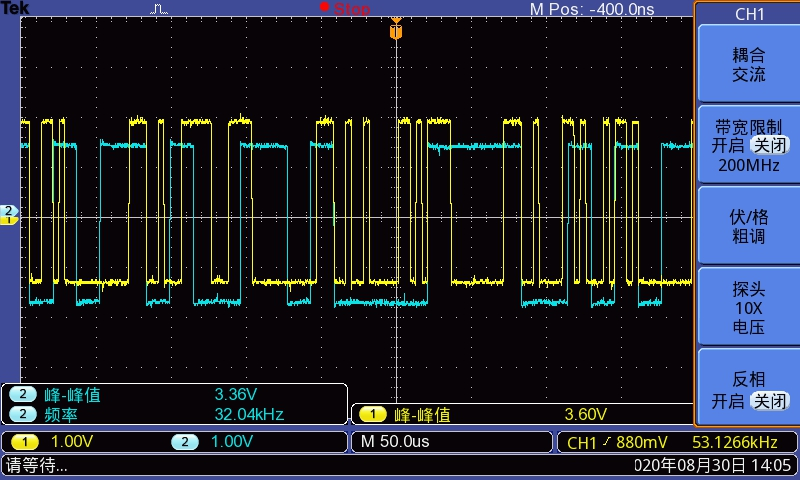
\includegraphics[
      width = \linewidth,
    ]{pcm/fm}
    \caption{PCM 复用前后}%
    \label{fig:pcm/fm}
  \end{subfigure}
  \quad
  \begin{subfigure}[htbp]{0.45\linewidth}
    \centering
    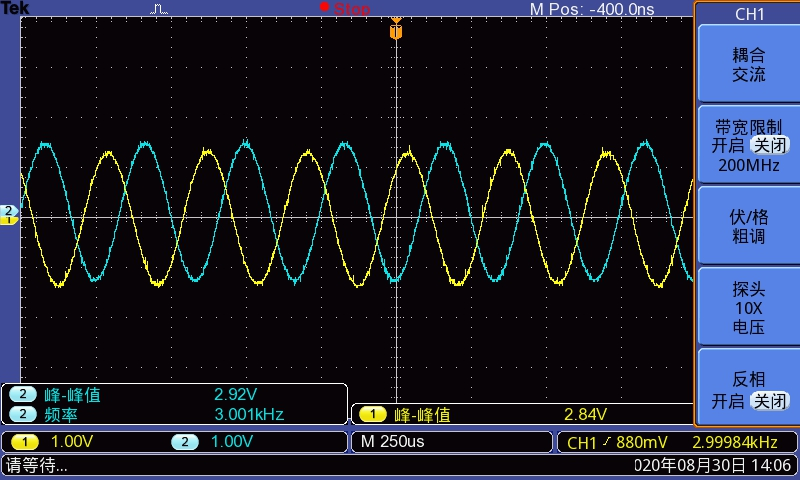
\includegraphics[
      width = \linewidth,
    ]{pcm/encode}
    \caption{PCM 编译码前后}%
    \label{fig:pcm/encode}
  \end{subfigure}
  \caption{PCM}%
  \label{fig:pcm}
\end{figure}

\subsection{2M 时分复用及解复用}%
\label{sub:2m}

% 该项目是设置菜单为复用速率为 2048KHz,实验观测的过程同 256K 的时分复用。

% \begin{enumerate}
%   \item 实验连线与 256K 时分复用及解复用的实验项目~\ref{sub:256k}相同。
%   \item 开电,设置主控菜单,选择【主菜单】→【通信原理】→【时分复用】→【复用速
%     率 2048KHz】。将模块 13 的 S3 拨位“0001”。将 21 号模块的开关 S1 拨至
%     A-LAW(或 U-LAW)。
%   \item 此时系统初始状态为:在复用时隙的速率 2048K 模式,7 号模块的复用信号共
%     有 32 个时隙;第 0 时隙数据为巴克码、第 1、2、3、4 时隙数据分别为 DIN1、
%     DIN2、DIN3、DIN4 端口的数据,开关 S1 拨码信号初始分配在第 5 时隙,通过主
%     控可以设置 7 号模块拨码开关 S1 数据的所在时隙位置。另外,此时信号源 A-OUT
%     输出 1KHz 的正弦波,幅度由 W1 可调(频率和幅度参数可根据主控模块操作说明
%     进行调节);PCM 数据送至 7 号模块的 DIN2 端口。
%   \item 实验操作及波形观测。
\begin{enumerate}
  \item 用示波器观测 2048M 复用输出信号。改变 7 号模块的拨码开关 S1,观测复
    用输出中信号变化情况图~\ref{fig:2048m}\footnote{拨码开关在第五时隙,可以
    看到第五时隙信号确实发生了变化}。
  \item 在主控菜单中选择“第 5 时隙加”图~\ref{fig:ts5/add}和“第 5 时隙减”
    图~\ref{fig:ts5/sub},观测拨码开关 S1 对应数据在复用输出信号中的所在帧位
    置变化情况\footnote{可以通过第5时隙加、减调整拨码开关输入的时隙位置}。
  \item 用示波器对比观测信号源 A-OUT 和 21 号模块的音频输出,观测信号的恢复
    情况图~\ref{fig:aout}\footnote{波形相同,时间上有半个周期的延迟}。
\end{enumerate}
% \end{enumerate}

\begin{figure}[htbp]
  \centering
  \begin{subfigure}[htbp]{0.45\linewidth}
    \centering
    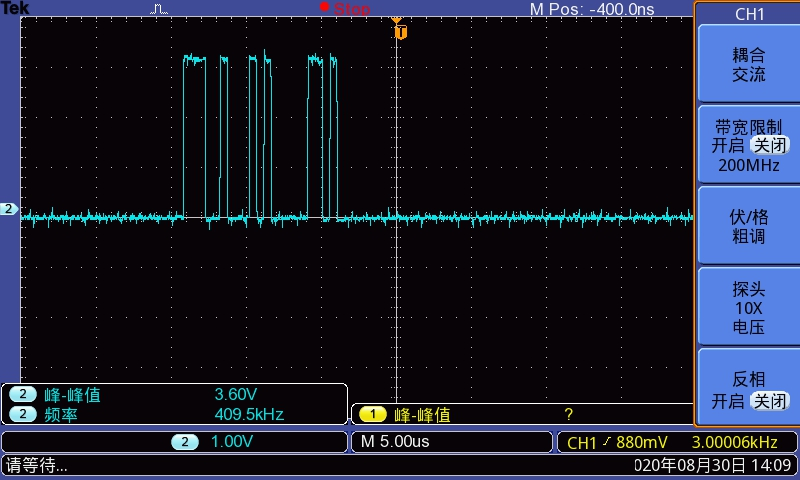
\includegraphics[
      width = \linewidth,
    ]{2048m/00000000}
    \caption{00000000}%
    \label{fig:2048m/00000000}
  \end{subfigure}
  \quad
  \begin{subfigure}[htbp]{0.45\linewidth}
    \centering
    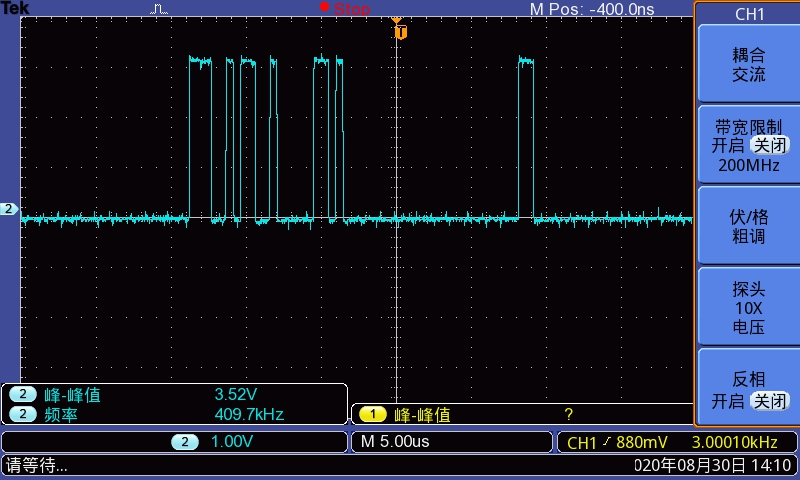
\includegraphics[
      width = \linewidth,
    ]{2048m/00000011}
    \caption{00000011}%
    \label{fig:2048m/00000011}
  \end{subfigure}

  \begin{subfigure}[htbp]{0.45\linewidth}
    \centering
    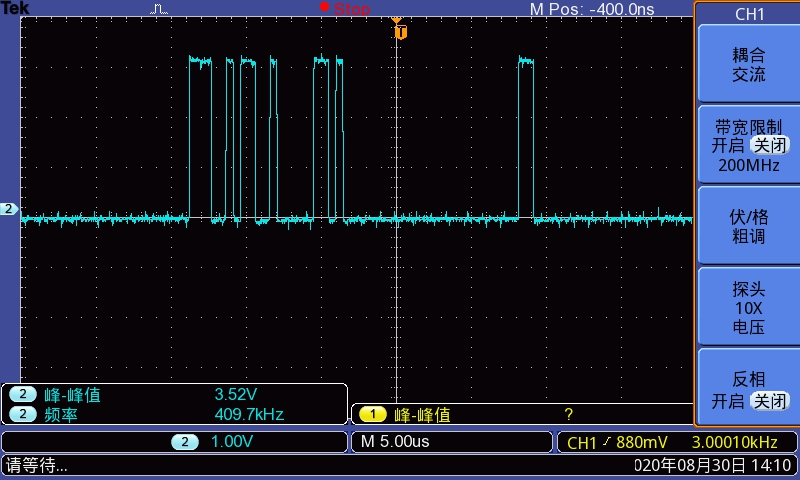
\includegraphics[
      width = \linewidth,
    ]{2048m/00000011}
    \caption{00011111}%
    \label{fig:2048m/00011111}
  \end{subfigure}
  \caption{改变 7 号模块的拨码开关 S1}%
  \label{fig:2048m}
\end{figure}

\begin{figure}[htbp]
  \centering
  \begin{subfigure}[htbp]{0.45\linewidth}
    \centering
    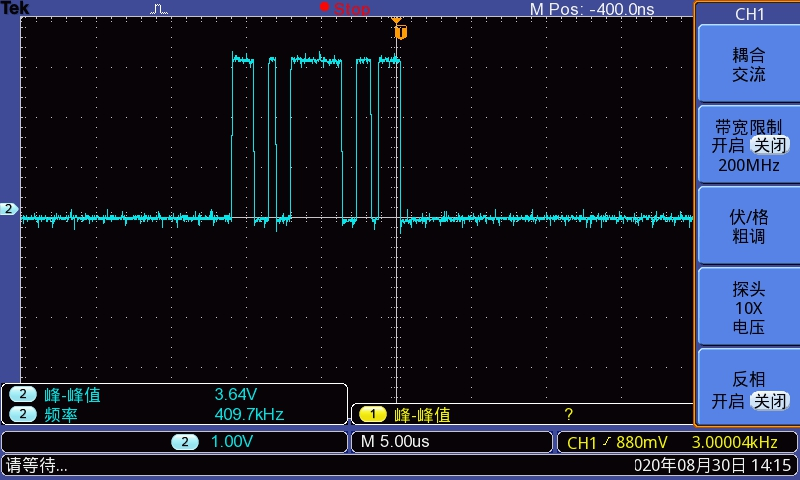
\includegraphics[
      width = \linewidth,
    ]{ts5/add}
    \caption{第 5 时隙加}%
    \label{fig:ts5/add}
  \end{subfigure}
  \quad
  \begin{subfigure}[htbp]{0.45\linewidth}
    \centering
    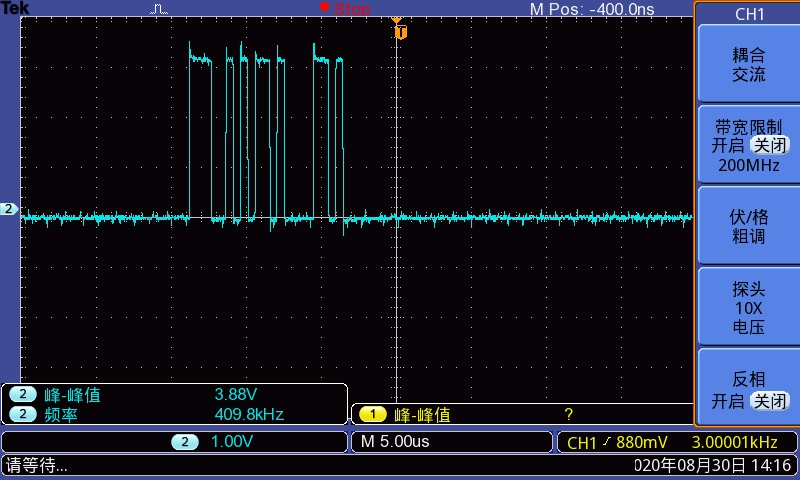
\includegraphics[
      width = \linewidth,
    ]{ts5/sub}
    \caption{第 5 时隙减}%
    \label{fig:ts5/sub}
  \end{subfigure}
  \caption{第 5 时隙}%
  \label{fig:ts5}
\end{figure}

\begin{figure}[htbp]
  \centering
  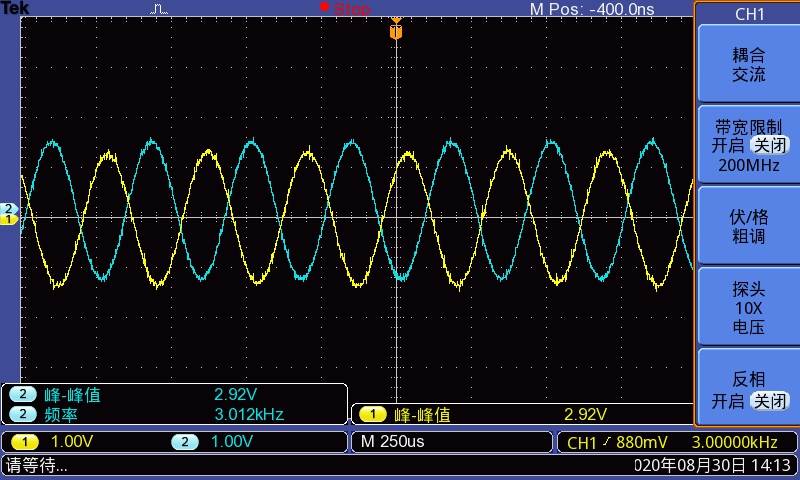
\includegraphics[
    width = 0.8\linewidth,
  ]{aout}
  \caption{信号源(蓝色)与音频输出}%
  \label{fig:aout}
\end{figure}

\section{实验报告}%
\label{sec:\arabic{chapter}report}

\begin{Exercise}
  画出各测试点波形,并分析实验现象。
\end{Exercise}

\begin{Answer}
  PCM 编译码前后波形图见图~\ref{fig:pcm/encode}。 PCM 复用前后波形图见
  图~\ref{fig:pcm/fm}。信号源(蓝色)与音频输出波形图见图~\ref{fig:aout}。

  分析:本实验主要观察了4路、32路频分复用和解复用的实验现象。256kHz 的时分复
  用1帧有4个时隙,分别是前面补0的巴克码、PN 15码、PCM 编码、拨码开关输入。
  2.048MHz 的时分复用1帧有 32 个时隙。(语音信号是 0.6--3.4kHz,为了防止混叠
  会留有一定余量,所以一般视为4kHz。采样后根据奈奎斯特采样定理变成8kHz,A 律
  PCM 编码后变成64kHz,4路频分复用后变成256kHz,32路频分复用成一个基群后变成
  2.048MHz。但注意的是本实验未涉及到更高的超群,由于群同步需要消耗一定的时间
  ,所以不再能用简单的乘法进行计算。)
\end{Answer}

\begin{Exercise}
  分析电路的工作原理,叙述其工作过程。
\end{Exercise}

\begin{Answer}
  实验电路的工作原理见图~\ref{fig:\arabic{chapter}dia},工作过程见
  章节~\ref{sec:\arabic{chapter}principle}。
\end{Answer}

\end{document}
